\section{Camada de Aplicação}

\subsection{Princípios da Camada de Rede}

    \textbf{Objetivos}

    \begin{itemize}[left=0.5cm, align=left, nosep]    
        \item Compreender aspectos conceituais e de implementação dos protocolos da camada de aplicação
        \begin{itemize}[left=0.5cm, nosep, label=$\hookrightarrow$]
            \item Modelos de serviço da \underline{camada de transporte}
            \item Paradigma \textbf{cliente-servidor}
            \item Paradigma \textbf{par a par} (peer-to-peer)
        \end{itemize}

        \item Aprender sobre protocolos por meio da análise dos protocolos populares da camada de aplicação e sua infraestrutura:   
         \begin{itemize}[left=0.5cm, nosep, label=$\hookrightarrow$]
            \item HTTP
            \item SMTP, IMAP
            \item DNS
            \item Sistemas de streaming de vídeo, CDNs
        \end{itemize}
    
        \item Programação de aplicações de rede:
        \begin{itemize}[left=0.5cm, nosep, label=$\hookrightarrow$]
            \item API de sockets
        \end{itemize}

    \end{itemize}  

    \textbf{Exemplos de Aplicativos de Rede}

    \vspace{-0.5cm}
    \begin{multicols}{2}
        \begin{itemize}[left=0.5cm, align=left, nosep]
            \item Redes Sociais
            \item Internet
            \item Mensagens de Texto
            \item E-mail
            \item Jogos online com vários usuários
            \item Transmissão de vídeo armazenado (YouTube, Hulu, Netflix)
            \item Compartilhamento de arquivos P2P
            \item Chamada sobre IP
            \item Videoconferência em tempo real (por exemplo, Zoom)
            \item Busca na Internet
            \item Acesso remoto
        \end{itemize}
    \end{multicols}

    \textbf{Criando um App de Rede}
    
    Escrevemos programas que:
    \begin{itemize}[left=0.5cm, align=left, nosep]
        \item Executem em diferentes sistemas finais.
        \item Se comuniquem pela rede.
        \item \underline{Exemplo:} O software de servidor web se comunica com o software de navegador.
    \end{itemize}

    Não há necessidade de escrever software para dispositivos do núcleo da rede
    \begin{itemize}[left=0.5cm, align=left, nosep]
        \item Dispositivos do núcleo da rede não executam aplicações de usuário.
        \item Aplicações em sistemas finais permitem o rápido desenvolvimento e a propagação de aplicativos.
    \end{itemize}

    \begin{figure}[H]
        \centering
        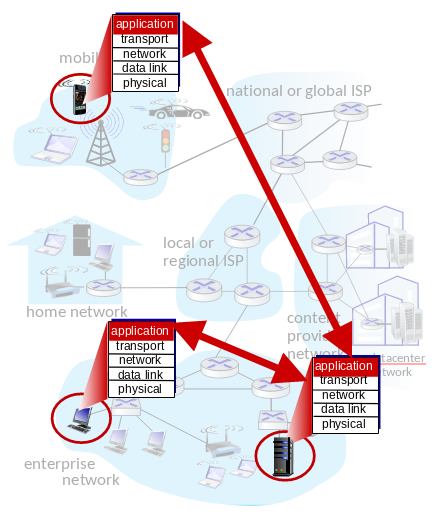
\includegraphics[width=0.27\textwidth]{img/02-camada-aplicacao/network-app}
    \end{figure}

    \textbf{Paradigma Cliente-Servidor}
    
    Servidor:
    \begin{itemize}[left=0.5cm, align=left, nosep]
        \item Host sempre ativo.
        \item Endereço IP permanente.
        \item Frequentemente em data centers, para fins de escalabilidade.
    \end{itemize}

    Cliente:
    \begin{itemize}[left=0.5cm, align=left, nosep]
        \item Contatar, comunicar-se com o servidor.
        \item Podem estar conectados de forma intermitente. 
        \item Podem ter endereços IP dinâmicos.
        \item Não se comunicam diretamente entre si.
        \item \underline{Exemplos:} HTTP, IMAP, FTP.
    \end{itemize}

    \begin{figure}[H]
        \centering
        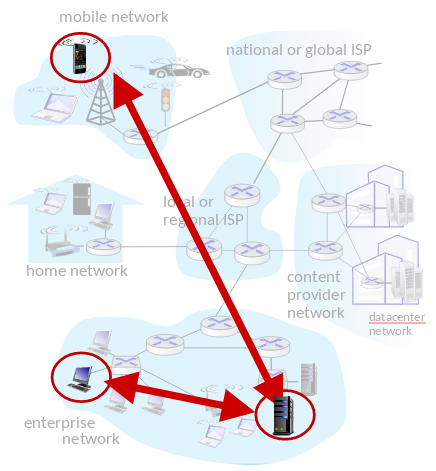
\includegraphics[width=0.3\textwidth]{img/02-camada-aplicacao/cliente-servidor}
    \end{figure}

    \textbf{Arquitetura Par a Par}
    \begin{itemize}[left=0.5cm, align=left, nosep]    
        \item Sem servidor sempre ativo.
        \item Sistemas finais arbitrários comunicam-se diretamente.
        \item Pares solicitam serviços a outros pares e, em contrapartida, prestam serviços a outros pares.
        \begin{itemize}[left=0.5cm, nosep, label=$\hookrightarrow$]
            \item \underline{Escalabilidade Intrínseca:} Novos pares trazem nova capacidade de serviço, bem como novas demandas de serviço.
        \end{itemize}  
        \item Pares conectam-se de forma intermitente e alteram seus endereços IP.
        \begin{itemize}[left=0.5cm, nosep, label=$\hookrightarrow$]
            \item Gerenciamento complexo $\ldots$
        \end{itemize} 
        \item \underline{Exemplo:} Compartilhamento de arquivos P2P [BitTorrent]
    \end{itemize} 

    \begin{figure}[H]
        \centering
        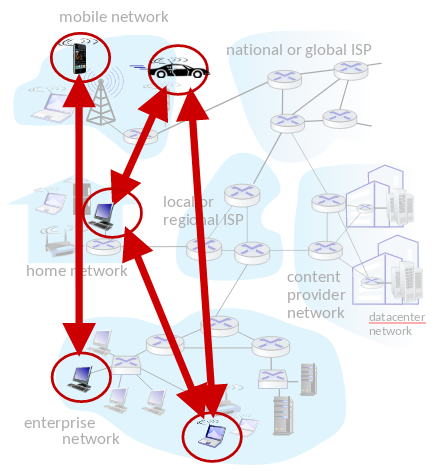
\includegraphics[width=0.3\textwidth]{img/02-camada-aplicacao/par-a-par}
    \end{figure}

    \textbf{Processos de Comunicação}
    \begin{itemize}[left=0.5cm, align=left, nosep]    
        \item \textbf{Processo:} programa em execução em um host.
        \item No mesmo host, dois processos comunicam-se utilizando \textbf{comunicação entre processos} (definida pelo SO).
        \item Processos em hosts diferentes comunicam-se por meio da troca de \textbf{mensagens}.
        \item \underline{Nota:} Aplicações com arquiteturas P2P possuem processos clientes e processos servidores.
        \begin{itemize}[left=0.5cm, nosep, label=$\hookrightarrow$]
            \item \textbf{Processo cliente:} Processo que inicia a comunicação.
            \item \textbf{Processo servidor:} Processo que aguarda ser contatado.
        \end{itemize}
    \end{itemize}

    \textbf{Sockets}
    \begin{itemize}[left=0.5cm, align=left, nosep]    
        \item O processo envia/recebe mensagens para/de seu \textbf{socket}.
        \item o socket é análogo a uma \underline{porta}:
        \begin{itemize}[left=0.5cm, nosep, label=$\hookrightarrow$]
            \item O processo remetente empurra a mensagem para fora pela porta.
            \item O processo remetente conta com a infraestrutura de transporte do outro lado da porta para entregar a mensagem 
            ao socket do processo receptor.
            \item Dois sockets envolvidos: um de cada lado.
        \end{itemize}  
    \end{itemize}  

    \begin{figure}[H]
        \centering
        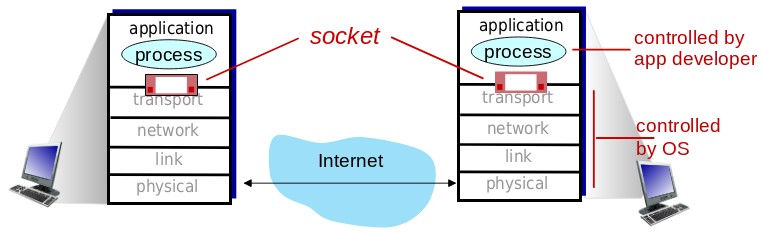
\includegraphics[width=0.5\textwidth]{img/02-camada-aplicacao/socket}
    \end{figure}

    \textbf{Processos de Endereçamento}
    \begin{itemize}[left=0.5cm, align=left, nosep]    
        \item Para receber mensagens, o processo precisa de um \textbf{identificador}.
        \item O dispositivo hospedeiro possui um endereço IP de 32 bits exclusivo.
        \item O endereço IP do host onde o processo é executado é não suficiente para identificar 
        o processo pois ários processos podem estar em execução no mesmo host.
        \item O \textbf{identificador} inclui tanto o \textbf{endereço IP} quanto os \textbf{números de porta} associados ao processo no hospedeiro.
        \item Exemplos de números de porta:
        \begin{itemize}[left=0.5cm, nosep, label=$\hookrightarrow$]
            \item Servidor HTTP: 80
            \item Servidor de email: 25
        \end{itemize}  
    \end{itemize}  

    \textbf{Um protocolo da camada de aplicação define:}
    \begin{itemize}[left=0.5cm, align=left, nosep]    
        \item \textbf{Tipos de mensagens} trocadas.
        \begin{itemize}[left=0.5cm, nosep, label=$\hookrightarrow$]
            \item \underline{Ex:} request (requisição), response (resposta).
        \end{itemize}  
        \item \textbf{Sintaxe da Mensagem:} Quais campos compõem as mensagens e como eles são delimitados.
        \item \textbf{Semântica da Mensagem:} Significado das informações nos campos.
        \item \textbf{Regras} sobre quando e como os processos enviam mensagens e respondem a elas.
        \item \textbf{Protocolos Abertos:}
        \begin{itemize}[left=0.5cm, nosep, label=$\hookrightarrow$]
            \item Definidos em RFCs; todos têm acesso à definição do protocolo.
            \item Permitem a interoperabilidade.
            \item \underline{Exemplo:} HTTP, SMTP.
        \end{itemize} 
        \item Protocolos Proprietários:
        \begin{itemize}[left=0.5cm, nosep, label=$\hookrightarrow$]
            \item \underline{Exemplo:} Zoom.
        \end{itemize} 
    \end{itemize}

    \textbf{Serviços de Transporte que um aplicativo/app precisa}
    \begin{itemize}[left=0.5cm, align=left, nosep]    
        \item \textbf{Integridade de Dados:}
        \begin{itemize}[left=0.5cm, nosep, label=$\hookrightarrow$]
            \item Algumas aplicações (por exemplo, transferência de arquivos, transações web) exigem transferência de dados 100\% confiável.
            \item Outras aplicações (por exemplo, áudio) podem tolerar alguma perda.
        \end{itemize}  
        \item \textbf{Timing/Temporização:}
        \begin{itemize}[left=0.5cm, nosep, label=$\hookrightarrow$]
            \item Alguns aplicativos (por exemplo, telefonia via Internet, jogos interativos) exigem baixa latência para serem ``eficazes''.
        \end{itemize}
        \item \textbf{Throughput/Vazão}
        \begin{itemize}[left=0.5cm, nosep, label=$\hookrightarrow$]
            \item Alguns aplicativos (por exemplo, multimídia) exigem uma taxa de transferência mínima para serem ``eficazes''.
            \item Outros aplicativos (``aplicativos elásticos'') utilizam qualquer taxa de transferência que lhes seja disponibilizada.
        \end{itemize}
        \item \textbf{Security/Segurança}
        \begin{itemize}[left=0.5cm, nosep, label=$\hookrightarrow$]
            \item Criptografia, Integridade dos dados $\ldots$
        \end{itemize}
    \end{itemize}

    \vspace{2cm}
    \textbf{Requisitos de Serviços de Transporte: Aplicativos Comuns}
    \begin{table}[ht]
        \centering
        \scriptsize
        \setlength{\tabcolsep}{3pt}

        \begin{tabular}{llll}
            \toprule
            \textbf{Aplicação} & \textbf{Perda} & \textbf{Taxa} & \textbf{Sensível ao atraso?} \\
            \midrule
            Transf./download de arquivos & Sem perda & Elástica & Não \\
            E-mail & Sem perda & Elástica & Não \\
            Documentos Web & Sem perda & Elástica & Não \\
            Áudio/vídeo em tempo real & Tol. à perda & Áudio: 5 Kbps--1 Mbps & Sim, dezenas de ms \\
            & & Vídeo: 10 Kbps--5 Mbps & \\
            Áudio/vídeo por streaming & Tol. à perda & Mesmo que acima & Sim, alguns segundos \\
            Jogos interativos & Tol. à perda & Kbps+ & Sim, dezenas de ms \\
            Mensagens de texto & Sem perda & Elástica & Sim e não \\
            \bottomrule
        \end{tabular}
    \end{table}

    \textbf{Serviços de Protocolos de Transporte da Internet}
    \begin{table}[ht]
        \centering
        \renewcommand{\arraystretch}{1.2}

        \begin{tabular}{p{0.47\textwidth} p{0.47\textwidth}}
            \toprule
            \textbf{Serviço TCP} & \textbf{Serviço UDP} \\
            \midrule

            \begin{itemize}[leftmargin=*,nosep]
                \item \textbf{Transporte confiável} entre os processos de envio e recepção;
                \item \textbf{Controle de fluxo:} O emissor não sobrecarrega o receptor;
                \item \textbf{Controle de congestionamento:} Reduz a taxa de envio quando a rede está congestionada;
                \item \textbf{Orientado à conexão:} Requer estabelecimento de conexão entre cliente e servidor;
                \item \textbf{Não fornece:} Garantias de tempo, vazão mínima ou segurança.
            \end{itemize}

            &

            \begin{itemize}[leftmargin=*,nosep]
                \item \textbf{Transferência de dados não confiável} entre os processos de envio e recepção;
                \item \textbf{Não fornece:} Confiabilidade, controle de fluxo, controle de congestionamento, garantias de tempo, vazão mínima, segurança ou estabelecimento de conexão.
            \end{itemize}

            \\
            \bottomrule
        \end{tabular}

    \end{table}

    \textbf{Exemplo: Aplicações de Internet e Protocolos de Transporte}
    \begin{table}[ht]
        \centering
        \footnotesize
        \setlength{\tabcolsep}{4pt}

        \begin{tabular}{lll}
            \toprule
            \textbf{Aplicação} & \textbf{Protocolo da aplicação} & \textbf{Protocolo de transporte} \\
            \midrule
            Transferência/download de arquivos & FTP (RFC 959) & TCP \\
            E-mail & SMTP (RFC 5321) & TCP \\
            Documentos Web & HTTP (RFC 7230, RFC 9110) & TCP \\
            Telefonia pela Internet &
            SIP (RFC 3261), RTP (RFC 3550) ou proprietário &
            TCP ou UDP \\
            Áudio/vídeo por streaming &
            HTTP (RFC 7230), DASH &
            TCP \\
            Jogos interativos &
            WOW, FPS (proprietário) &
            UDP ou TCP \\
            \bottomrule
        \end{tabular}

    \end{table}
    
    \textbf{Segurança no TCP}
    \begin{itemize}[left=0.5cm, align=left, nosep]    
        \item Vanilla TCP e UDP sockets:
        \begin{itemize}[left=0.5cm, nosep, label=$\hookrightarrow$]
            \item Sem criptografia.
            \item Senhas em \underline{texto simples/claro} enviadas pelo socket trafegam pela Internet em \underline{texto simples/claro} (!)
        \end{itemize}  
        \item Transport Layer Security (TLS):
        \begin{itemize}[left=0.5cm, nosep, label=$\hookrightarrow$]
            \item Fornece conexões TCP criptografadas.
            \item Integridade de dados.
            \item Autenticação de pontos finais.
        \end{itemize} 
        \item TLS é implementado na camada de aplicação.
        \begin{itemize}[left=0.5cm, nosep, label=$\hookrightarrow$]
            \item Aplicações utilizam bibliotecas TLS, que por sua vez utilizam TCP.
            \item Dados em \underline{texto simples/claro} enviados para o ``socket'' atravessam a Internet criptografados.
        \end{itemize} 
    \end{itemize}

\subsection{Web e HTTP}

    \begin{itemize}[left=0.5cm, align=left, nosep]    
        \item Uma página da Web consiste em \textbf{objetos}, cada um dos quais pode estar armazenado em servidores Web diferentes.
        \item Um objeto pode ser um arquivo HTML, uma imagem JPEG, um applet Java, um arquivo de áudio, $\ldots$
        \item Uma página da Web consiste em um \textbf{arquivo HTML base} que inclui \textbf{vários objetos referenciados}, \textbf{cada} um endereçável por uma \textbf{URL}.
        
        \[
        \underbrace{\text{\texttt{www.someschool.edu}}}_{\text{Host name}}
        \underbrace{\text{\texttt{/someDept/pic.gif}}}_{\text{Path name}}
        \]
    
    \end{itemize}  

    \textbf{HTTP: hypertext transfer protocol}
    \begin{itemize}[left=0.5cm, align=left, nosep]    
        \item Protocolo Web da camada de aplicação.
        \item Modelo cliente/servidor:
        \begin{itemize}[left=0.5cm, nosep, label=$\hookrightarrow$]
            \item \textbf{Cliente:} Navegador que solicita (\textit{requests}), recebe (usando o protocolo HTTP) e ``exibe'' objetos da Web.
            \item \textbf{Servidor:} Servidor Web que envia (usando o protocolo HTTP) objetos em resposta (\textit{response}) a solicitações (\textit{requests}).
        \end{itemize}  
    \end{itemize} 

    \begin{figure}[H]
        \centering
        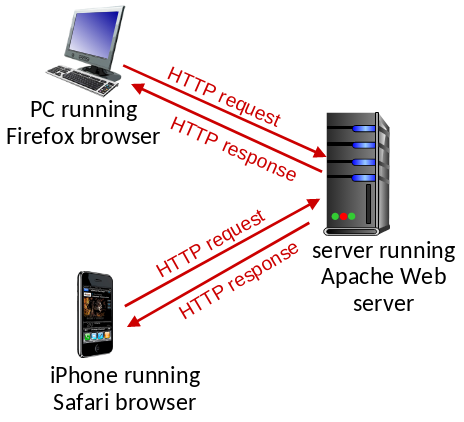
\includegraphics[width=0.4\textwidth]{img/02-camada-aplicacao/http}
    \end{figure}
    
    \textbf{O HTTP utiliza TCP:}
    \begin{itemize}[left=0.5cm, align=left, nosep]    
        \item O cliente inicia uma conexão TCP (cria um socket) com o servidor, na porta 80.
        \item O servidor aceita a conexão TCP do cliente.
        \item Mensagens HTTP (mensagens do protocolo da camada de aplicação) são trocadas entre o navegador (cliente HTTP) e o servidor Web (servidor HTTP).
        \item A conexão TCP é encerrada.
    \end{itemize}  

    \vspace{0.5cm}
    \textbf{O HTTP é ``sem estado'' (\textit{stateless})}
    \begin{itemize}[left=0.5cm, align=left, nosep]    
        \item O servidor não mantém informações sobre solicitações anteriores do cliente.
        \item \textbf{Obs: Protocolos que mantêm o "estado" são complexos!}
        \begin{itemize}[left=0.5cm, nosep, label=$\hookrightarrow$]
            \item O histórico anterior (estado) precisa ser mantido.
            \item Se o servidor ou o cliente falhar, suas visões do ``estado'' podem ficar inconsistentes e precisam ser reconciliadas.
        \end{itemize} 
    \end{itemize} 

    \textbf{Conexões HTTP: Dois Tipos}
    \begin{itemize}[left=0.5cm, align=left, nosep]    
        \item \textbf{HTTP não persistente (\textit{Non-persistent HTTP})}
        \begin{itemize}[left=0.5cm, nosep, label=$\hookrightarrow$]
            \item Conexão TCP aberta.
            \item No máximo um objeto enviado pela conexão TCP.
            \item Conexão TCP fechada.
            \item \textbf{Obs:} O download de múltiplos objetos exigia múltiplas conexões.
        \end{itemize}  
        
        \item \textbf{HTTP Persistente (\textit{Persistent HTTP})}
         \begin{itemize}[left=0.5cm, nosep, label=$\hookrightarrow$]
            \item Conexão TCP aberta com um servidor.
            \item Múltiplos objetos podem ser enviados por meio de uma única conexão TCP entre o cliente e esse servidor.
            \item Conexão TCP encerrada.
        \end{itemize}
    \end{itemize}

    \textbf{HTTP não persistente: Exemplo}
    \begin{figure}[H]
        \centering
        \begin{minipage}{0.53\textwidth}
            \centering
            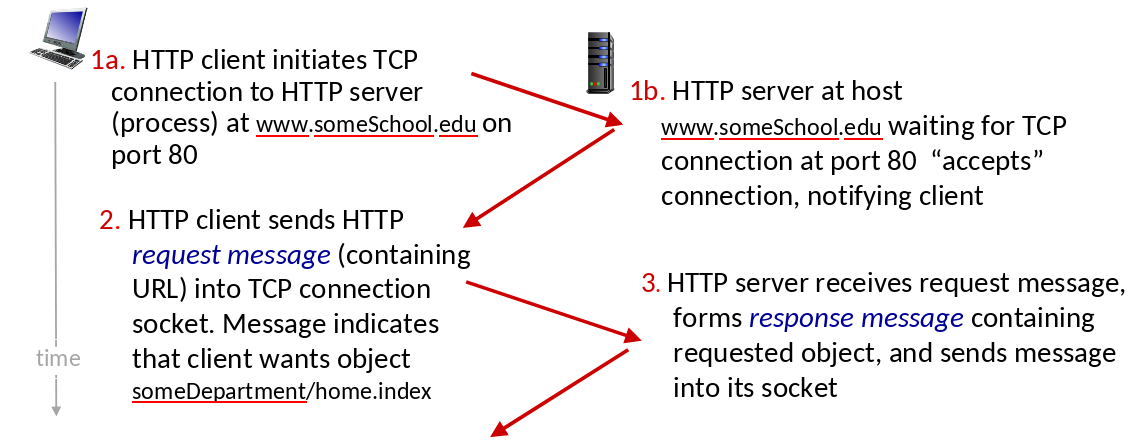
\includegraphics[width=\linewidth]{img/02-camada-aplicacao/http-nao-persistente-01}
        \end{minipage}
        \hfill
        \begin{minipage}{0.42\textwidth}
            \centering
            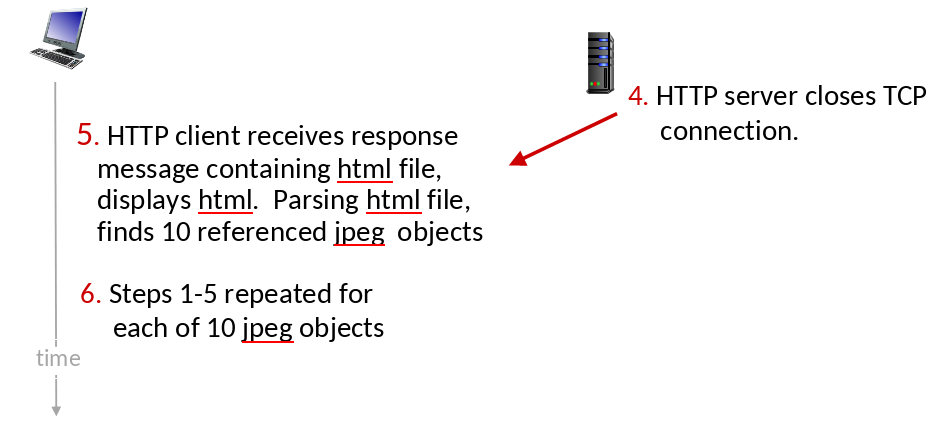
\includegraphics[width=\linewidth]{img/02-camada-aplicacao/http-nao-persistente-02}
        \end{minipage}
    \end{figure}

    \textbf{HTTP não persistente: Tempo de Resposta}
    \begin{itemize}[left=0.5cm, align=left, nosep]    
        \item \textbf{RTT:} Tempo para um pacote pequeno viajar do cliente ao servidor e retornar.
        \item \textbf{Tempo de resposta HTTP/\textit{HTTP response time} (por objeto):}
        \begin{itemize}[left=0.5cm, nosep, label=$\hookrightarrow$]
            \item Um RTT para iniciar a conexão TCP.
            \item Um RTT para a requisição HTTP e o retorno dos primeiros bytes da resposta HTTP.
            \item Tempo de transmissão do objeto/arquivo.
        \end{itemize}  
    \end{itemize}
    
    Tempo de resposta do HTTP não persistente = 2 RTT + tempo de transmissão do arquivo

    \begin{figure}[H]
        \centering
        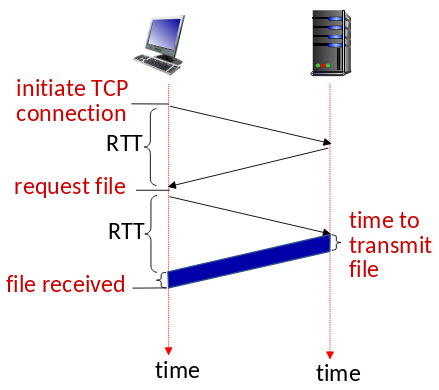
\includegraphics[width=0.25\textwidth]{img/02-camada-aplicacao/tempo-de-resposta}
    \end{figure}


    \textbf{HTTP Persistente (HTTP 1.1)}
    \begin{itemize}[left=0.5cm, align=left, nosep]    
        \item \textbf{Problemas do HTTP não persistente:}
        \begin{itemize}[left=0.5cm, nosep, label=$\hookrightarrow$]
            \item Requer 2 RTTs por objeto.
            \item Sobrecarga do SO para cada conexão TCP.
            \item Navegadores frequentemente abrem múltiplas conexões TCP paralelas para buscar objetos referenciados em paralelo.
        \end{itemize}  
        \item \textbf{HTTP Persistente (HTTP 1.1):}
        \begin{itemize}[left=0.5cm, nosep, label=$\hookrightarrow$]
            \item O servidor mantém a conexão aberta após enviar a resposta.
            \item Mensagens HTTP subsequentes entre o mesmo cliente e servidor são enviadas pela conexão aberta.
            \item O cliente envia requisições assim que encontra um objeto referenciado.
            \item Apenas um RTT para todos os objetos referenciados (reduzindo o tempo de resposta pela metade).
        \end{itemize} 
    \end{itemize}

    \textbf{Mensagem de \textit{request}(solicitação) HTTP}
    \begin{itemize}[left=0.5cm, align=left, nosep]    
        \item Dois tipos de mensagens HTTP: \textbf{request(\textit{requisição}), response(\textit{resposta}).}
        \item \textbf{HTTP request message:} ASCII
        \begin{itemize}[left=0.5cm, nosep, label=$\hookrightarrow$]
            \item Formato legível por humanos.
        \end{itemize}  
        
        \begin{figure}[H]
            \centering
            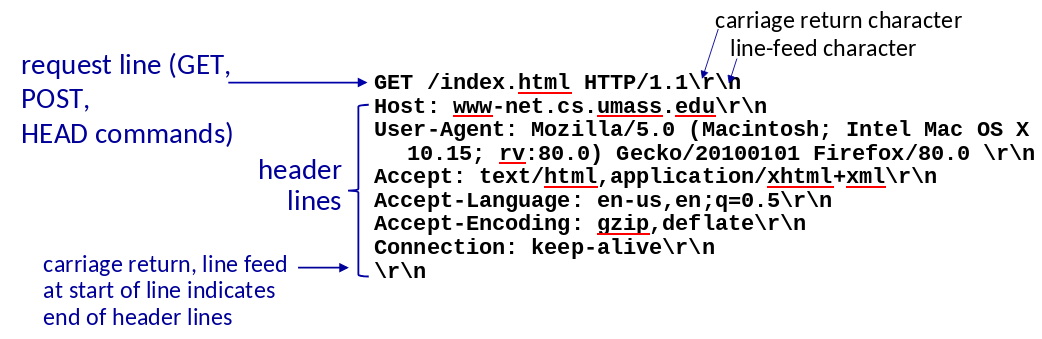
\includegraphics[width=0.7\textwidth]{img/02-camada-aplicacao/request-message}
        \end{figure}
    
    \end{itemize}

    \textbf{Formato General da Mensagem}
    \begin{figure}[H]
        \centering
        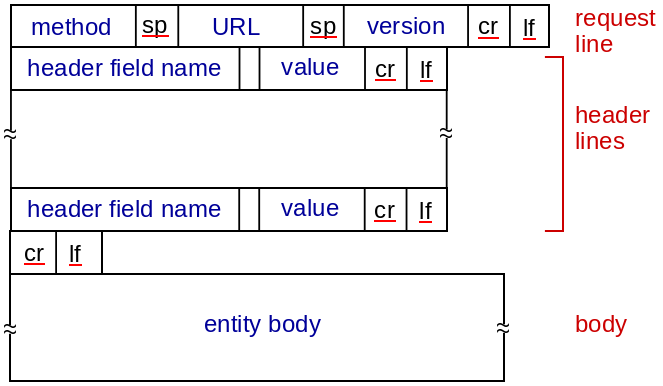
\includegraphics[width=0.5\textwidth]{img/02-camada-aplicacao/request-message-formato}
    \end{figure}
    
    \textbf{Outras \textit{request messages} (mensagens de solicitação) HTTP}
    \begin{itemize}[left=0.5cm, align=left, nosep]    
        \item \textbf{Método \underline{POST}:}
        \begin{itemize}[left=0.5cm, nosep, label=$\hookrightarrow$]
            \item Uma página da web frequentemente inclui campos de formulário.
            \item A entrada do usuário é enviada do cliente para o servidor no corpo da entidade de uma mensagem de requisição HTTP POST.
        \end{itemize} 
        \vspace{0.5cm}
        \item \textbf{Método \underline{GET}:} Para enviar dados ao servidor
        \begin{itemize}[left=0.5cm, nosep, label=$\hookrightarrow$]
            \item Incluir dados do usuário no campo URL da mensagem de requisição HTTP GET (após um `?'):
            \item \texttt{www.somesite.com/animalsearch?monkeys\&banana}
        \end{itemize} 
        \item \textbf{Método \underline{HEAD}:}
        \begin{itemize}[left=0.5cm, nosep, label=$\hookrightarrow$]
            \item Solicita apenas os cabeçalhos (\textit{headers}) que seriam retornados se a URL especificada fosse requisitada com o método HTTP GET.
        \end{itemize} 
        \item \textbf{Método \underline{PUT}:}
        \begin{itemize}[left=0.5cm, nosep, label=$\hookrightarrow$]
            \item Faz o upload de um novo arquivo (objeto) para o servidor.
            \item Substitui completamente o arquivo existente na URL especificada pelo conteúdo do corpo da entidade da mensagem de requisição HTTP POST.
        \end{itemize}  
    \end{itemize}  

    \textbf{HTTP response message}
    \begin{figure}[H]
        \centering
        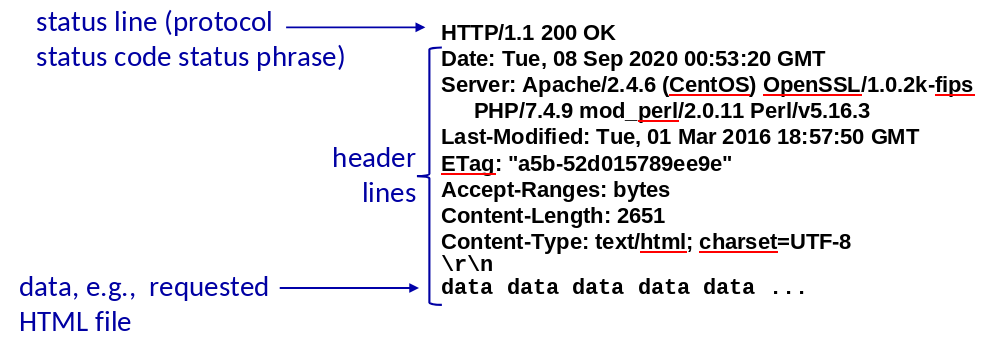
\includegraphics[width=0.5\textwidth]{img/02-camada-aplicacao/response-message}
    \end{figure}
    
    \textbf{HTTP response status codes}
    \begin{itemize}[left=0.5cm, align=left, nosep]    
        \item O código de status aparece na primeira linha da mensagem de resposta do servidor para o cliente.
        \item \textbf{200 OK}
        \begin{itemize}[left=0.5cm, nosep, label=$\hookrightarrow$]
            \item Solicitação/requisição bem-sucedida; objeto solicitado mais adiante nesta mensagem.
        \end{itemize}
        \item \textbf{301 Moved Permanently}
        \begin{itemize}[left=0.5cm, nosep, label=$\hookrightarrow$]
            \item O objeto solicitado foi movido; a nova localização está especificada mais adiante nesta mensagem (no campo \textit{Location:}).
        \end{itemize}
        \item \textbf{400 Bad Request}
        \begin{itemize}[left=0.5cm, nosep, label=$\hookrightarrow$]
            \item \underline{Mensagem} de solicitação (\textit{request message}) não compreendida pelo servidor.
        \end{itemize}
        \item \textbf{404 Not Found}
        \begin{itemize}[left=0.5cm, nosep, label=$\hookrightarrow$]
            \item Documento solicitado não encontrado neste servidor.
        \end{itemize}
        \item \textbf{505 HTTP Version Not Supported}
    \end{itemize}

    \textbf{Manutenção do estado do usuário/servidor: cookies}
    \begin{itemize}[left=0.5cm, align=left, nosep]    
        \item Lembre-se: a interação HTTP GET/resposta é \textbf{sem estado}.
        \item Não há noção de trocas de mensagens HTTP em várias etapas para concluir uma ``transação'' na Web.
        \begin{itemize}[left=0.5cm, nosep, label=$\hookrightarrow$]
            \item Não há necessidade de o cliente/servidor rastrear o ``estado'' de uma troca em várias etapas.
            \item Todas as solicitações HTTP são independentes umas das outras.
            \item Não há necessidade de o cliente/servidor ``se recuperar'' de uma transação parcialmente concluída, mas nunca totalmente finalizada.
        \end{itemize}  
        \item Um protocolo \textbf{\textit{stateful}} (com estado): o cliente faz duas alterações em X, ou nenhuma.
        
        \begin{figure}[H]
        \centering
            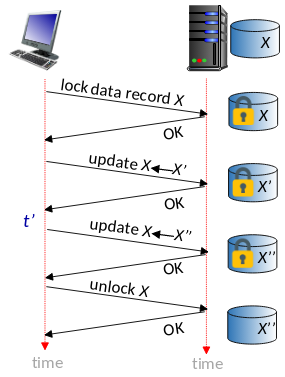
\includegraphics[width=0.3\textwidth]{img/02-camada-aplicacao/cookies-exemplo01}
        \end{figure}
    
    \end{itemize}  

    Sites e navegadores de clientes utilizam \textbf{cookies} para manter um estado entre transações.

    \textbf{Quatro Componentes:}
    \begin{enumerate}[left=0.5cm, align=left, nosep]
        \item Linha de cabeçalho de cookie da mensagem de resposta HTTP (\textit{HTTP response message}).
        \item Linha de cabeçalho de cookie na próxima mensagem de requisição HTTP (\textit{HTTP request message})..
        \item Arquivo de cookie armazenado no host do usuário, gerenciado pelo navegador do usuário.
        \item Banco de dados de back-end no site
    \end{enumerate}

    \textbf{Exemplo:}
    \begin{itemize}[left=0.5cm, align=left, nosep]    
        \item Susan usa o navegador em seu notebook e acessa um site de e-commerce específico pela primeira vez.
        \item Quando as requisições HTTP iniciais chegam ao site, este cria:
        \begin{itemize}[left=0.5cm, nosep, label=$\hookrightarrow$]
            \item Um ID exclusivo (também conhecido como ``cookie'').
            \item Uma entrada no banco de dados de \underline{backend} para esse ID.
        \end{itemize}
        \item As requisições HTTP subsequentes de Susan para esse site conterão o valor do ID do cookie, permitindo que o site ``identifique'' Susan.
        
        \begin{figure}[H]
        \centering
            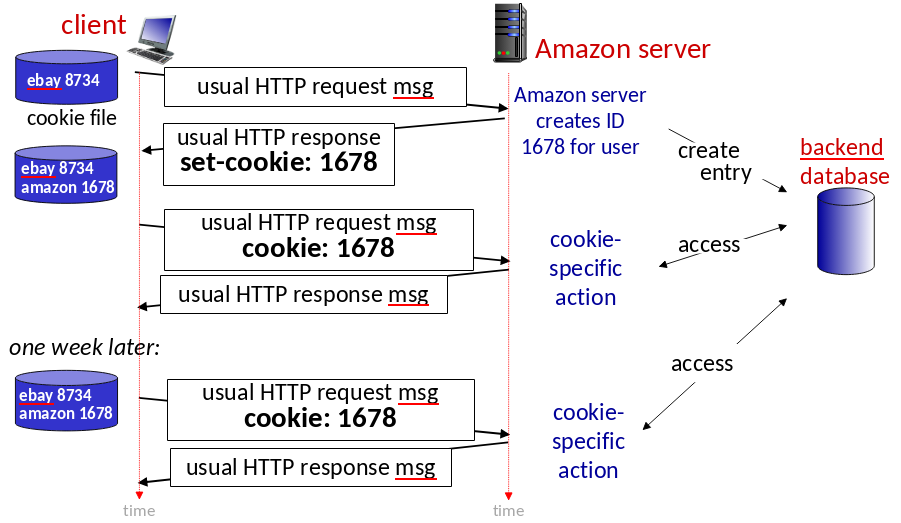
\includegraphics[width=0.6\textwidth]{img/02-camada-aplicacao/cookies-exemplo02}
        \end{figure}
    
    \end{itemize} 

    \textbf{HTTP cookies: Comentários}
    \begin{itemize}[left=0.5cm, align=left, nosep]    
        \item Em que os cookies podem ser usados ?
        \begin{itemize}[left=0.5cm, nosep, label=$\hookrightarrow$]
            \item Autorização
            \item Carrinhos de Compra
            \item Recomendações
            \item Estado da sessão do usuário (Webmail)
        \end{itemize}
        \item Desafio: Como manter o estado ?
        \begin{itemize}[left=0.5cm, nosep, label=$\hookrightarrow$]
            \item \textbf{Nos \textit{endpoints} do protocolo:} Manter o estado no Emissor/receptor ao longo de múltiplas transações.
            \item \textbf{Nas mensagens:} cookies em mensagens HTTP carregam o estado.
        \end{itemize}  
        \item \textbf{cookies e privacidade:}
        \begin{itemize}[left=0.5cm, nosep, label=$\hookrightarrow$]
            \item Os cookies permitem que os sites obtenham muitas informações sobre você durante a sua visita.
            \item cookies persistentes de terceiros (cookies de rastreamento) permitem que uma identidade comum (valor do cookie) seja rastreada em vários sites.
        \end{itemize} 
    \end{itemize}


\subsection{E-mail, SMTP, IMAP}
\subsection{DNS: Domain Name System}
\subsection{Streaming de Vídeo e Distribuição de Conteúdo na Internet}
\subsection{Programação de Socket com UDP e TCP}

    \textbf{dasd}

    \begin{itemize}[left=0.5cm, align=left, nosep]    
        \item dasd
        \begin{itemize}[left=0.5cm, nosep, label=$\hookrightarrow$]
            \item po
        \end{itemize}  
    \end{itemize}  

    \begin{figure}[H]
        \centering
        %\includegraphics[width=0.5\textwidth]{img/02-camada-aplicacao/}
    \end{figure}
